\documentclass[12pt,a4paper]{article}

\usepackage{mathtools}
\usepackage{graphicx}
\usepackage{braket}
\usepackage{amsthm}
\usepackage{lmodern}
\usepackage[utf8]{inputenc}
\usepackage[frenchb]{babel}
\usepackage[T1]{fontenc}
\usepackage{subcaption}
\usepackage{caption}
\usepackage{gensymb}
\usepackage{tikz}
\usepackage{qcircuit}
\usepackage{listings}
\usepackage{pgfplots}
\usepackage{appendix}
\usepackage{hyperref}
\usepackage[ruled,vlined]{algorithm2e}
\usepackage{titlesec}
\usepackage{cleveref}
\usepackage{titling}
\usepackage{float}

\newtheorem{definition}{Définition}
\newtheorem{pb}{Problème}
\newtheorem{rem}{Remarque}
\newtheorem{ex}{Exemple}
\setlength{\droptitle}{-10em}

\title{Recuit Quantique}
\date{}

\begin{document}
\maketitle

\section{Opérateur Hamiltonien}
\subsection*{Modèle d'Ising}
Posons trois aimants $\{\sigma_1, \sigma_2, \sigma_3\}$ et notons $+1$ si ils indiquent \textit{Nord} et $-1$ si ils indiquent \textit{Sud}, par exemple:  "N - S - N" donne $\{+1, -1, +1\}$. L'énergie du système est alors la somme des interactions, donné par l'opérateur Hamiltonien. Dans le cas d'exemple, on aurait: $\mathcal{H} = \sigma_1 \sigma_2 + \sigma_2 \sigma_3$. On peut alors généraliser:  

$\mathcal{H} = \displaystyle\sum_{<i, j>} \sigma_i \sigma_j$, avec les $<i, j>$ paires d'aimants.

Maintenant, supposons qu'on puisse contrôler la force d'interaction entre les aimants. Cela introduit un nouveau terme $J_{ij}$ représentant cette force d'interaction. On peut alors écrire: 

$\mathcal{H} = \displaystyle\sum_{<i, j>} J_{ij} \sigma_i \sigma_j$.

Ensuite, on rajoute un champ magnétique global au système. Cela rajoute une interaction $h_i$ à chaque aimant $i$, on rajoute donc la somme des $h_i \sigma_i$ à l'expression. Par convention, on inverse les signes: 

$\mathcal{H} = -\displaystyle\sum_{<i, j>} J_{ij} \sigma_i \sigma_j - \displaystyle\sum_{i} h_i \sigma_i $.

On a donc les $J_{ij}$ représentant la force d'interaction entre les aimants, ou le \textit{couplage} du système, et les $h_i$ représentant le champ magnétique, ou le \textit{biais} du système.

On peut représenter l'énergie du système par un graphe, comme à la figure \ref{fig:energyGraph}: 

\begin{figure}[H]
    \centering
    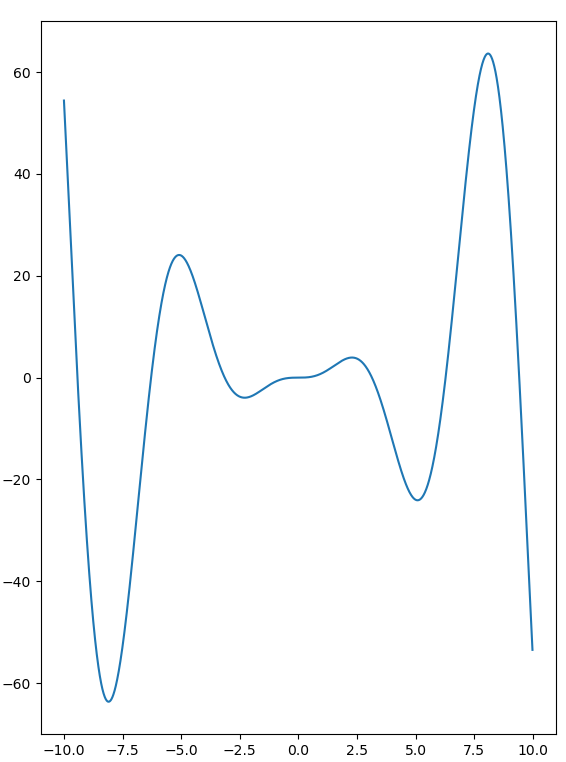
\includegraphics[scale=0.2]{ex_energy_graph.png}
    \caption{Exemple de graphe d'énergie}
    \label{fig:energyGraph}
\end{figure}


Naturellement, le système va tendre vers un état d'énergie minimum. En revanche, il peut se retrouver dans un minimum local, et ne pas avoir assez d'énergie pour sauter vers un état d'énergie plus bas.


\section{Recuit Quantique}
\subsection*{Principe général}
Le recuit quantique est l'analogue de la simulation de recuit en classique. A la place des gradients de température utilisés en classique pour passer d'un minimum local à un autre, on utilise en quantique la possibilité des systèmes quantiques de faire des sauts d'états, permettant potentiellement d'éviter de se retrouver bloqué dans un minimum local.

Dans le recuit quantique, on considère que la fonction de coût correspond à trouver l'état de base d'un Hamiltonien d'Ising $\mathcal{H}_0$ (vecteur d'état propre de $\mathcal{H}_0$ ayant la plus faible énergie). L'idée est de constituer un Hamiltonien évoluant au cours du temps:

\begin{equation}
    \mathcal{H}(t) = A(t) \mathcal{H}_0 + B(t) \mathcal{H}_1.
\end{equation}

Au départ, on aura $B(t) = 0$ et $A(t) = 1$. En faisant évoluer le système, on obtient à la fin de l'évolution $B(t) = 1$ et $A(t) = 0$. Cela permet donc au système de passer progressivement du premier Hamiltonien $\mathcal{H}_1$ vers l'Hamiltonien d'Ising $\mathcal{H}_0$.

Tout d'abord, pour appliquer l'Hamiltonien d'Ising à un système quantique, on doit ré-écrire son équation pour transformer les termes individuels $\sigma_i$ en des matrices de Pauli Z $\sigma_i^z = \begin{bmatrix} 1 & 0 \\ 0 & -1 \\ \end{bmatrix}$:

\begin{equation}
    \mathcal{H}_0 = -\displaystyle\sum_{<i, j>} J_{ij} \sigma_i^z \sigma_j^z - \displaystyle\sum_{i} h_i \sigma_i^z.
\end{equation}

Comme cet Hamiltonien final correspond au modèle d'Ising classique, uniquement composé de matrices de Pauli Z (donc commutable), son état de base encode le résultat du problème.

\medbreak

On écrit ensuite l'Hamiltonien utilisé au départ:

\begin{equation}
    \mathcal{H}_1 = - \displaystyle\sum_{i} g_i \sigma_i^x.
\end{equation}

On introduit ici la matrice de Pauli X de façon à avoir un système non-commutable au cours de l'évolution quand $\mathcal{H}(t)$ est composé à la fois de $\mathcal{H}_0$ et de $\mathcal{H}_1$. On utilise cet Hamiltonien car son état de base correspond à l'état superposé équiprobable, qui nous est facile à créer.

Il est aussi possible de ré-écrire cette équation en changeant le terme d'évolution du temps: on utilise alors $s = \frac{t}{T}$ :

\begin{equation}
    \mathcal{H}_0 = - A(s) (\displaystyle\sum_{i} g_i \sigma_i^x ) - B(s) ( \displaystyle\sum_{<i, j>} J_{ij} \sigma_i^z \sigma_j^z + \displaystyle\sum_{i} h_i \sigma_i^z ).
    \label{eq:eq4}
\end{equation}

\subsection*{Théorème adiabatique quantique}
L'évolution d'un système quantique au cours du temps nous est donné par l'équation de Schrödinger:

\begin{equation}
    i \frac{d}{dt} \ket{\psi(t)} = \mathcal{H}(t) \ket{\psi(t)},
\end{equation}

où $\ket{\psi(t)}$ est le vecteur d'état dépendant du temps, et $\mathcal{H}(t)$ est l'Hamiltonien dépendant du temps. Pour chaque temps $t$, l'Hamiltonien $\mathcal{H}(t)$ possède un vecteur d'état de base $\ket{\psi_g (t)}$ étant le vecteur d'état propre ayant la plus faible énergie.

Le théorème adiabatique stipule que si $\mathcal{H}(t)$ évolue suffisament lentement, alors le vecteur d'état évoluant $\ket{\psi(t)}$ va rester proche du vecteur de base $\ket{\psi_g (t)}$.

On peut alors caractériser la performance du recuit quantique par le gap d'énergie entre l'état d'énergie minimale, et le premier état excité dans l'Hamiltonien intermédiaire. En revenant à l'équation \ref{eq:eq4}, on peut prendre en exemple $A(s) = (1 - \frac{t}{T})$ et $B(s) = \frac{t}{T}$. Dans ce cas, on peut indiquer que $T \in \mathcal{O}( \frac{1}{g_{min}^2})$, avec $g_{min}$ gap minimal pour $\mathcal{H}(t)$.

\subsection*{Approximation de l'évolution adiabatique}
En pratique, on peut implémenter une évolution adiabatique au moyen d'un circuit quantique. Cette implémentation passe dans un premier temps par la discrétisation de l'évolution $\mathcal{H}_0 \to \mathcal{H}_1$. La deuxième étape [...]

\medbreak

\begin{definition}
    Si on pose $\mathcal{H}(t)$ et $\mathcal{H}'(t)$ deux opérateurs Hamiltoniens, dépendant du temps, avec $t \in [0, T]$. On pose $U(t)$ et $U'(t)$ leurs évolutions unitaires respectives. Si on a $|| \mathcal{H}(t) - \mathcal{H}'(t) || < \delta$ pour chaque $t$, alors la différence des transformations est aussi bornée: $||U(t) - U'(t)|| \leq  \sqrt{2T\delta}$.
    \label{def:1}
\end{definition}



On peut alors discrétiser l'évolution $\mathcal{H}_0 \to \mathcal{H}_1$ à $H'_1, H'_2, \dots, H'_r$, chacun étant appliqué pendant $\frac{T}{r}$. On peut alors poser $U'(T) = e^{-i (\frac{T}{r}) \mathcal{H}'_r} \dots e^{-i (\frac{T}{r}) \mathcal{H}'_1}$, avec $\mathcal{H}'_j = \mathcal{H}(\frac{jT}{r}) = (1 - \frac{j}{r}) \mathcal{H}_0 + (\frac{j}{r}) \mathcal{H}_1$. On aura alors une faible différence, suivant la borne $\delta$ définie en \ref{def:1}.


\subsection*{Formulation du problème du voyageur de commerce en modèle QUBO}

Le problème du voyageur de commerce peut se formuler avec un Hamiltonien combinaison de deux Hamiltoniens élémentaires, celui pour les problèmes de cycles (dirigés ou non), avec l'ajout de la notion de coût du chemin.

\begin{equation}
    \mathcal{H}_A = A \displaystyle \sum_{v=1}^{n} (1 - \displaystyle \sum_{i=1}^{n} x_ {v,i})^2 + A \displaystyle \sum_{i=1}^{n} (1 - \displaystyle \sum_{iv=1}^{n} x_ {v,i})^2,
\end{equation}

pour l'énergie des problèmes de cycles, avec le premier terme indiquant qu'un n\oe ud n'apparait qu'une seule fois dans le trajet, et le deuxième terme indiquant qu'il doit y avoir un $j^{ème}$ n\oe ud dans le cycle pour chaque $j$.

\begin{equation}
    \mathcal{H}_B = B \displaystyle \sum_{uv \in E} W_{uv} \displaystyle \sum_{j=1}^{n} x_{u,j}x_{u,j+1},
\end{equation}

pour l'énergie correspondant au poids entre les n\oe uds, avec la distance ou le poids indiqué par le coefficient $W_{uv}$. On peut alors définir $\mathcal{H}_{TSP} = \mathcal{H}_A + \mathcal{H}_B$ l'opérateur Hamiltonien pour le problème de voyageur de commerce. \`A noter, on effectue ici les sommes sur les $n$ n\oe uds (villes) du problème, car on veut pouvoir retourner au point de départ (indice $j+1$ dans la dernière somme). On peut considérer également qu'on s'arrête à $n-1$ si on ne veut pas fermer le cycle.

\end{document}
